\documentclass[../DoAn.tex]{subfiles}
\begin{document}

Chương này trình bày cách hiện thực các thành phần đã thiết kế ở
Chương~\ref{chapter:Design}: môi trường triển khai, giai đoạn phân tích
tĩnh, giai đoạn phân tích động, pipeline tích hợp và giao diện web demo.

\section{Môi trường triển khai}
\label{section:4.1}

Hệ thống chạy trên hai nút phân tách: máy chủ vật lý cài
Kali Linux đóng vai host điều phối, và máy ảo Windows~10 22H2
x64 đóng vai guest thực thi mẫu. Bảng~\ref{tab:env-hardware}
liệt kê các thông số cấu hình của từng nút.
\begin{table}[H]
\centering
\caption{Cấu hình phần cứng và phần mềm môi trường triển khai.}
\label{tab:env-hardware}
\begin{tabular}{|l|l|l|}
\hline
\multicolumn{1}{|c|}{\textbf{Thành phần}} & \multicolumn{1}{c|}{\textbf{Thông số}} & \multicolumn{1}{c|}{\textbf{Giá trị}} \\
\hline
Máy chủ (host) & CPU                    & AMD Ryzen 7 8845HS \\
               & RAM                    & 32 GB \\
               & Hệ điều hành           & Kali Linux \\
               & Nền tảng ảo hóa        & VirtualBox \\
               & Mạng giả lập           & INetSim \\
               & Thời gian chờ khởi động & 120 giây \\
               & Cửa sổ quan sát (mặc định) & 120 giây \\
\hline
Máy ảo (guest) & vCPU                   & 4 \\
               & RAM                    & 4 GB \\
               & Hệ điều hành           & Windows~10 22H2 x64 \\
               & Tên VM                 & \texttt{win10} \\
               & Snapshot sạch          & \texttt{Clean\_Base} \\
               & Địa chỉ IP             & \texttt{192.168.56.106} \\
               & Sysmon                 & v15.x (schema~4.90) \\
               & SilkETW                & v8 \\
               & Agent HTTP             & FastAPI, cổng~\texttt{8001} \\
\hline
\end{tabular}
\end{table}
Máy chủ vật lý cài Kali Linux điều phối toàn bộ vòng đời guest
qua \texttt{VBoxManage}: khôi phục snapshot trước mỗi phiên, truyền
tệp mẫu, truy vấn trạng thái Agent, rồi tắt máy khi phiên kết thúc.
Pipeline viết bằng Python; giai đoạn phân tích tĩnh thực hiện trực
tiếp trên host, song song với quan sát động ở guest.

\subsection{Máy ảo Windows}
\label{section:4.1.2}

Máy ảo chạy Windows~10 22H2 x64, đặt tên \texttt{win10} trong
VirtualBox. Trước mỗi phiên, pipeline phục hồi snapshot
\texttt{Clean\_Base} để đưa guest về trạng thái nguyên vẹn, nhanh
hơn tái khởi động và loại bỏ dữ liệu tồn dư từ mẫu trước.

Ba công cụ được nhúng sẵn trong snapshot: Sysmon~v15 ghi các sự kiện
tiến trình, mạng, registry và tệp; SilkETW~v8 thu sự kiện ETW từ
\texttt{Microsoft-Windows-DotNETRuntime} để bắt hoạt động .NET; và
Agent (FastAPI, cổng~\texttt{8001}) làm điểm nhận lệnh từ host. Sau
khi guest khởi động, host thăm dò \texttt{/health} tối đa 120 giây
để xác nhận Agent đã sẵn sàng nhận lệnh.
Hình~\ref{fig:vm-virtualbox} minh họa cấu hình phần cứng máy ảo.
\begin{figure}[H]
\centering
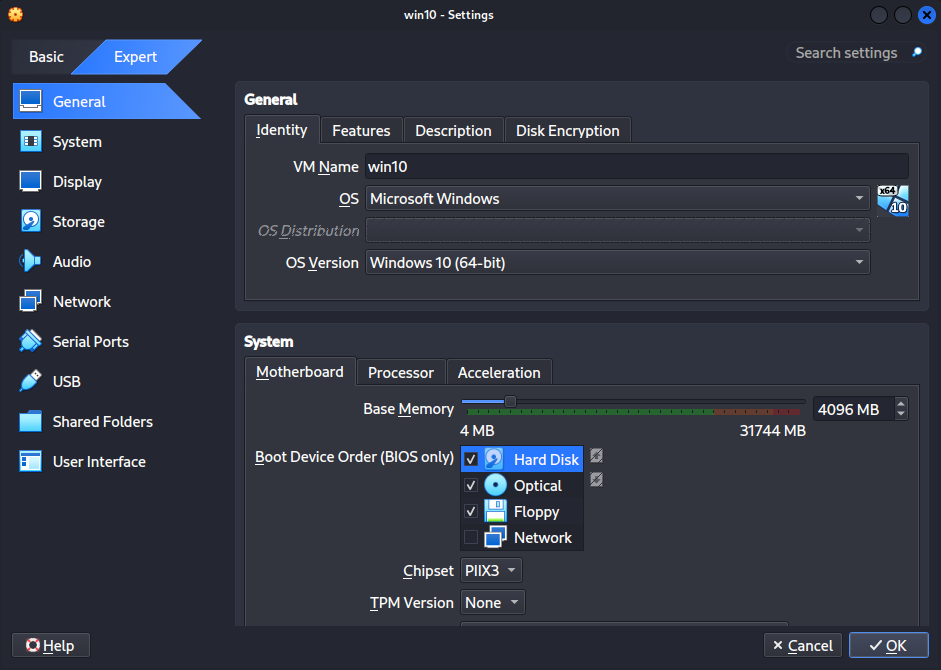
\includegraphics[width=0.78\textwidth]{Hinhve/Pic16VM_VirtualBox.png}
\caption{Cấu hình phần cứng máy ảo \texttt{win10} trong VirtualBox Settings.}
\label{fig:vm-virtualbox}
\end{figure}
\subsection{Cấu hình mạng và INetSim}
\label{section:4.1.3}

Adapter mạng guest ở chế độ host-only (IP tĩnh
\texttt{192.168.56.106}), không có kết nối trực tiếp ra Internet.
INetSim chạy trên host giả lập DNS, HTTP/HTTPS và TCP để duy trì
luồng thực thi mẫu mà không phát sinh lưu lượng ra mạng thực tế.
Hình~\ref{fig:host-only-network} trình bày cấu hình adapter mạng
host-only trong VirtualBox Settings.
\begin{figure}[H]
\centering
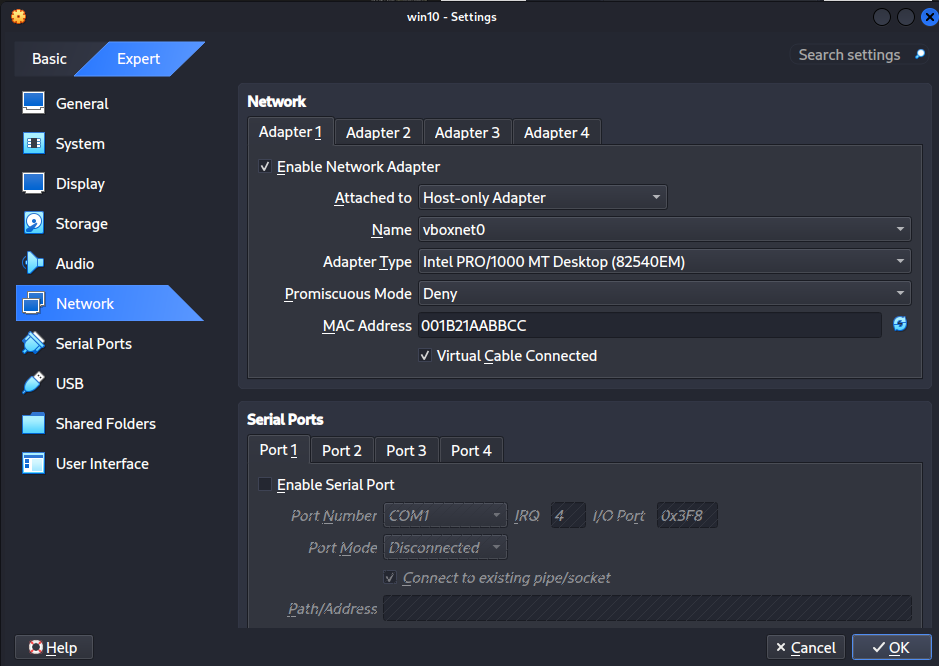
\includegraphics[width=0.8\textwidth]{Hinhve/Pic17Host_only.png}
\caption{Cấu hình adapter mạng host-only của máy ảo trong VirtualBox Settings.}
\label{fig:host-only-network}
\end{figure}
\section{Triển khai giai đoạn phân tích tĩnh}
\label{section:4.2}

\subsection{Thu thập và xây dựng tập dữ liệu}
\label{section:4.2.1}

Phần lành tính gồm 110.002 tệp PE thu thập từ tám phiên bản
Windows và các nguồn phần mềm hợp pháp (Chocolatey, Sysinternals,
Nirsoft và các bản phát hành mã nguồn mở trên GitHub); phần mã độc
gồm 132.476 tệp từ VirusShare~\cite{virusshare} và
MalwareBazaar~\cite{malwarebazaar} thuộc nhiều họ phổ biến như
AgentTesla, AsyncRAT, Emotet, STOP và nhiều họ khác. Thống kê chi
tiết theo từng nguồn được trình bày tại Phụ lục A.1 và A.2.
Do khối lượng hàng trăm nghìn mẫu, quá trình xây dựng tập huấn
luyện được chia làm hai bước, trong đó bước đầu xử lý theo lô để
kiểm soát mức sử dụng bộ nhớ.

Bước 1 — Trích xuất theo lô. Tệp PE được xử lý riêng
theo từng nhãn bằng cơ chế lô 50 mẫu: kiểm tra chữ ký MZ, loại
trùng lặp theo SHA-256, trích xuất vector 2.381 chiều và ghi tệp
tạm sau mỗi lô để có thể tiếp tục nếu gián đoạn; sau khi duyệt
hết, các lô được hợp nhất thành ma trận lành tính và mã độc riêng.
Hình~\ref{fig:process-data} minh họa quy trình xây dựng từng
tập theo nhãn ở bước này.
\begin{figure}[H]
\centering
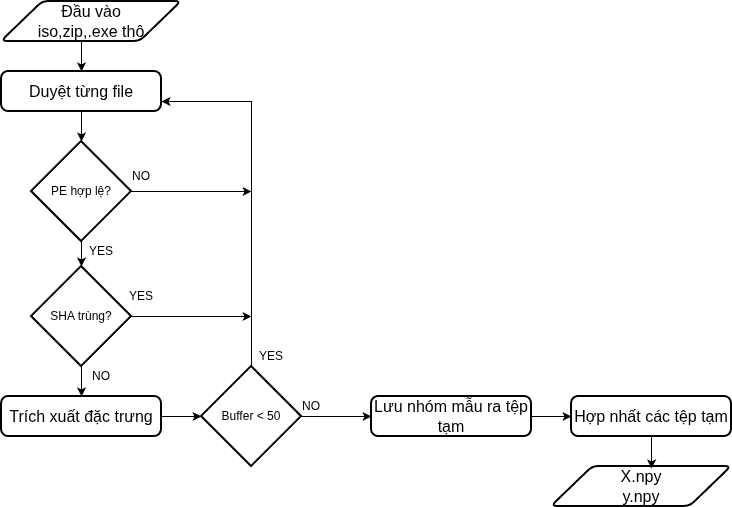
\includegraphics[width=1.0\textwidth]{Hinhve/Pic9Proccessdata.png}
\caption{Sơ đồ quá trình xây dựng ma trận đặc trưng từ tệp PE thô.}
\label{fig:process-data}
\end{figure}
Bước 2 — Ghép, xáo trộn và tiền xử lý. Hai ma trận được
nối theo hàng rồi xáo trộn với seed cố định ($seed = 42$). Tập kết
hợp sau đó được làm sạch: lọc bỏ nhãn ngoài $\{0, 1\}$; điền giá
trị NaN/Inf bằng trung vị theo đặc trưng; loại trùng lặp theo MD5
của từng dòng vector; xáo trộn lại lần cuối. Kết quả ghi đè
\texttt{X\_final.npy} và \texttt{y\_final.npy} để dùng cho huấn luyện.

Bảng~\ref{tab:dataset-final} trình bày thành phần tập dữ liệu
huấn luyện sau ba bước xử lý trên.
\begin{table}[H]
\centering
\caption{Thành phần tập dữ liệu huấn luyện cuối cùng
  (\texttt{X\_final.npy}, 2.381 đặc trưng/mẫu).}
\label{tab:dataset-final}
\begin{tabular}{|l|r|r|}
\hline
\multicolumn{1}{|c|}{\textbf{Nhãn}} & \multicolumn{1}{c|}{\textbf{Số mẫu}} & \multicolumn{1}{c|}{\textbf{Tỉ lệ}} \\
\hline
Lành tính (benign)  & 100.668 & 49{,}9\% \\
\hline
Mã độc (malware)    & 100.972 & 50{,}1\% \\
\hline
\textbf{Tổng}       & \textbf{201.640} & \textbf{100\%} \\
\hline
\end{tabular}
\end{table}
\subsection{Trích xuất đặc trưng}
\label{section:4.2.2}

Bộ trích xuất được hiện thực theo thiết kế tại
Mục~\ref{section:3.3.2}, dùng thư viện \texttt{pefile} để phân tích
cấu trúc PE. Mỗi tệp được biểu diễn bằng một vector 2.381 chiều ---
hiểu đơn giản là một dãy 2.381 con số, mỗi số là giá trị của một đặc
trưng --- ghép từ chín nhóm đặc trưng EMBER
(Bảng~\ref{tab:ember_features} ở Chương~\ref{chapter:Related_works}).

Phần lớn đặc trưng là các giá trị số có sẵn trong cấu trúc PE (kích
thước tệp, entropy từng section, các trường header, tần suất byte\ldots)
nên được điền thẳng vào vector. Khó khăn nằm ở các nhóm chứa danh sách
tên có độ dài thay đổi giữa các tệp --- tên thư viện và hàm import, tên
hàm export, tên section: số lượng tên mỗi tệp một khác nên không thể
xếp trực tiếp vào số ô cố định. Feature hashing giải quyết việc này:
một hàm băm ánh xạ mỗi tên tới một vị trí cố định trong mảng rồi cộng
dồn vào vị trí đó, nhờ vậy dù một tệp import 5 hay 500 hàm, đầu ra vẫn
là vector cùng số chiều. Cụ thể, tên thư viện import được băm vào 256
vị trí, cặp (thư viện, hàm) import vào 1.024 vị trí, tên hàm export vào
128 vị trí và tên section vào 50 vị trí. Tệp thiếu bảng import hoặc
export cho vector toàn 0 ở nhóm tương ứng.

Bộ trích xuất chạy trên 242.478 tệp PE thô và tạo ra 201.640 vector
hợp lệ. Tệp hợp lệ là tệp PE đúng định dạng, được \texttt{pefile} đọc
thành công để tính đủ chín nhóm đặc trưng; phần còn lại bị loại vì
không phải PE thật (thiếu chữ ký PE) hoặc có cấu trúc bị hỏng, cắt cụt
nên không đọc được.
\subsection{Huấn luyện và lưu mô hình}
\label{section:4.2.3}

Lần huấn luyện thứ nhất — lựa chọn thuật toán.
Ba thuật toán Random Forest, XGBoost và LightGBM được huấn luyện
độc lập trên 161.312 mẫu (80\%, seed~$= 42$) và đánh giá trên
40.328 mẫu kiểm thử chung, đảm bảo kết quả khác biệt đến từ bản
chất thuật toán. Siêu tham số của từng thuật toán được trình bày
trong Bảng~\ref{tab:fullmodel-params}.
\begin{table}[H]
\centering
\caption{Siêu tham số ba thuật toán trong lần huấn luyện thứ
  nhất (toàn bộ 2.381 đặc trưng, tập train 161.312 mẫu).}
\label{tab:fullmodel-params}
\begin{tabular}{|l|c|c|c|}
\hline
\multicolumn{1}{|c|}{\textbf{Siêu tham số}} & \multicolumn{1}{c|}{\textbf{Random Forest}} & \multicolumn{1}{c|}{\textbf{XGBoost}} & \multicolumn{1}{c|}{\textbf{LightGBM}} \\
\hline
Số cây / vòng tối đa     & 500    & 1.000   & 1.000 \\
\hline
Chiều sâu tối đa         & 15     & 15      & 15 \\
\hline
Tỉ lệ đặc trưng sử dụng & 0{,}8  & 0{,}8   & 0{,}8 \\
\hline
Mẫu tối thiểu mỗi lá    & 20     & 20      & --- \\
\hline
Tốc độ học               & ---    & 0{,}05  & 0{,}05 \\
\hline
Số lá tối đa             & ---    & ---     & 1.024 \\
\hline
Early stopping           & ---    & 50 vòng & 50 vòng \\
\hline
\end{tabular}
\end{table}
Kết quả so sánh trên tập kiểm thử nội bộ
(Chương~\ref{chapter:Experiment}) cho thấy LightGBM đạt hiệu
năng tốt nhất và được chọn cho lần huấn luyện thứ hai. Chỉ số
Importance Gain của mô hình này được dùng để xếp hạng 2.381 đặc
trưng theo đóng góp vào khả năng phân loại; ba tập chỉ số ứng với
$N \in \{128, 256, 384\}$ đặc trưng có đóng góp cao nhất được lưu
lại theo ba ngưỡng tham chiếu từ Choudhary et~al.~\cite{choudhary2025}.

Lần huấn luyện thứ hai — lựa chọn tập con đặc trưng.
Để định vị số chiều cần thiết, số đặc trưng được khảo sát trên lưới
mười lăm mốc từ 8 đến 2.381: mỗi mốc rút gọn dữ liệu theo bộ chỉ số
tương ứng và huấn luyện LightGBM một lần với cùng siêu tham số, cho ra
đường hiệu năng theo số chiều dùng tại Mục~\ref{section:5.2.2}. Riêng
ba ngưỡng tham chiếu 128, 256 và 384 được huấn luyện đầy đủ hơn bằng
5-fold Stratified Cross-Validation (seed~$= 42$), giữ lại fold đạt
AUC-ROC cao nhất làm mô hình đại diện; Bảng~\ref{tab:domainmodel-params}
trình bày siêu tham số sử dụng.
\begin{table}[H]
\centering
\caption{Siêu tham số LightGBM trong lần huấn luyện thứ hai
  (tập con đặc trưng, 5-fold CV trên 201.640 mẫu).}
\label{tab:domainmodel-params}
\begin{tabular}{|l|c|}
\hline
\multicolumn{1}{|c|}{\textbf{Siêu tham số}} & \multicolumn{1}{c|}{\textbf{Giá trị}} \\
\hline
Tốc độ học               & 0{,}05 \\
\hline
Số lá tối đa             & 512 \\
\hline
Chiều sâu tối đa         & 12 \\
\hline
Tỉ lệ đặc trưng sử dụng & 0{,}8 \\
\hline
Số vòng tối đa           & 600 \\
\hline
Early stopping           & 30 vòng \\
\hline
\end{tabular}
\end{table}
Kết quả so sánh bốn mô hình trên tập EMBER~2024 được trình bày tại
Chương~\ref{chapter:Experiment}. Mô hình Top-384 được chọn tích hợp
vào pipeline; khi suy luận, mô hình nhận vector 2.381 chiều, rút gọn
xuống 384 chiều theo bộ chỉ số đã lưu rồi trả về nhãn và xác suất
malware. Ngưỡng phân loại $\tau$ được xác định qua phân tích đánh đổi
FPR/FNR, trình bày tại Chương~\ref{chapter:Experiment}.

\section{Triển khai giai đoạn phân tích động}
\label{section:4.3}

\subsection{Cấu hình Sysmon}
\label{section:4.3.1}

Sysmon~v15 (schema~4.90) được nhúng sẵn vào snapshot
\texttt{Clean\_Base} nên không cần cài lại sau mỗi phiên. Hệ
thống đọc trực tiếp kênh \texttt{Microsoft-Windows-Sysmon/Operational}
qua PowerShell, ghi lại số thứ tự sự kiện (\texttt{RecordId}) mới
nhất làm mốc trước khi mẫu chạy; mỗi vòng lặp 100~ms chỉ lấy sự
kiện có \texttt{RecordId} lớn hơn mốc và chuyển đổi sang JSON, đảm
bảo đầu ra chỉ chứa sự kiện phát sinh trong phiên hiện tại. Phạm vi
giám sát được thu hẹp về cây tiến trình của mẫu: bộ thu thập theo
dõi PID gốc và tự động bổ sung PID con; sự kiện từ PID ngoài danh
sách bị bỏ qua. Danh sách 23~Event ID được liệt kê tại Phụ lục B.1
(Bảng~\ref{tab:sysmon-eids}).

Hình~\ref{fig:sysmon-eventlog} cho thấy các sự kiện Sysmon thô trên
kênh \texttt{Microsoft-Windows-Sysmon/Operational} trong Windows Event
Viewer.
\begin{figure}[H]
\centering
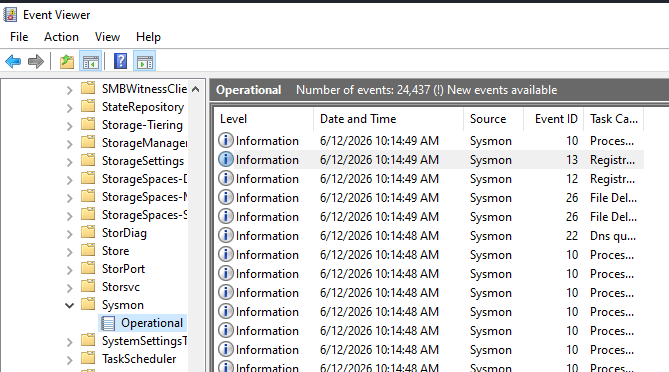
\includegraphics[width=\linewidth]{Hinhve/Pic19WindowEvent.png}
\caption{Kênh sự kiện \texttt{Microsoft-Windows-Sysmon/Operational}
  trong Windows Event Viewer.}
\label{fig:sysmon-eventlog}
\end{figure}
Trên guest, tập lệnh \path{start_collector.ps1} đọc kênh Sysmon và ghi
từng sự kiện thô ra tệp \texttt{sysmon\_events.jsonl} trong thư mục log
của phiên; lớp Bridge trên host kéo tệp này về qua endpoint
\texttt{/read} của Agent (Mục~\ref{section:4.3.3}) để đưa vào bước
chuẩn hóa. Hình~\ref{fig:sysmon-jsonl} trình bày nội dung thô của tệp
\texttt{sysmon\_events.jsonl} sau khi kéo về host.
\begin{figure}[H]
\centering
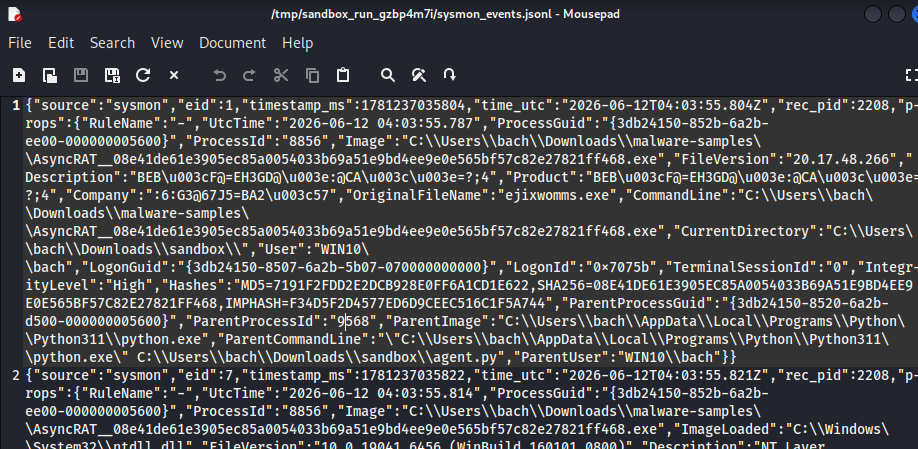
\includegraphics[width=\linewidth]{Hinhve/Pic20SysmonJsonl.png}
\caption{Các sự kiện Sysmon thô trong tệp \texttt{sysmon\_events.jsonl}
  sau khi kéo từ guest về host.}
\label{fig:sysmon-jsonl}
\end{figure}
\subsection{Cấu hình SilkETW}
\label{section:4.3.2}
SilkETW~v8 cũng được nhúng sẵn trong snapshot. Provider
\texttt{Microsoft-Windows-DotNETRuntime} với bộ lọc
\texttt{Method/LoadVerbose} bổ sung khả năng quan sát hoạt động
nạp assembly .NET mà Sysmon không ghi nhận ở mức hệ điều hành;
thông tin namespace và phương thức thu được phục vụ nhận diện
assembly đáng ngờ ở bước chuẩn hóa. Bảng~\ref{tab:silketw-params}
liệt kê các tham số cấu hình.
\begin{table}[H]
\centering
\caption{Tham số cấu hình SilkETW trong mỗi phiên phân tích.}
\label{tab:silketw-params}
\begin{tabular}{|l|l|}
\hline
\multicolumn{1}{|c|}{\textbf{Tham số}} & \multicolumn{1}{c|}{\textbf{Giá trị}} \\
\hline
Chế độ thu thập  & User-mode (\texttt{-t user}) \\
\hline
Provider         & \texttt{Microsoft-Windows-DotNETRuntime} \\
\hline
Bộ lọc sự kiện  & Tên sự kiện = \texttt{Method/LoadVerbose} \\
\hline
Kiểu đầu ra      & Tệp JSON (\texttt{-ot file}) \\
\hline
Tệp đầu ra       & \texttt{etw\_dotnet.json} \\
\hline
Thời gian chạy   & Bằng cửa sổ quan sát (mặc định 120 giây) \\
\hline
\end{tabular}
\end{table}
Cả hai tác vụ được khởi động đồng thời bởi cùng một script
\path{start_collector.ps1} trên guest; SilkETW dừng tự động khi hết
cửa sổ quan sát và ghi các sự kiện thô ra tệp \texttt{etw\_dotnet.json}.
Tương tự tệp Sysmon, tệp này được lớp Bridge kéo từ guest về host qua
endpoint \texttt{/read} của Agent (Mục~\ref{section:4.3.3}) để đưa vào
bước chuẩn hóa. Hình~\ref{fig:silketw-output} cho thấy nội dung thô của
tệp \texttt{etw\_dotnet.json} sau một phiên quan sát.
\begin{figure}[H]
\centering
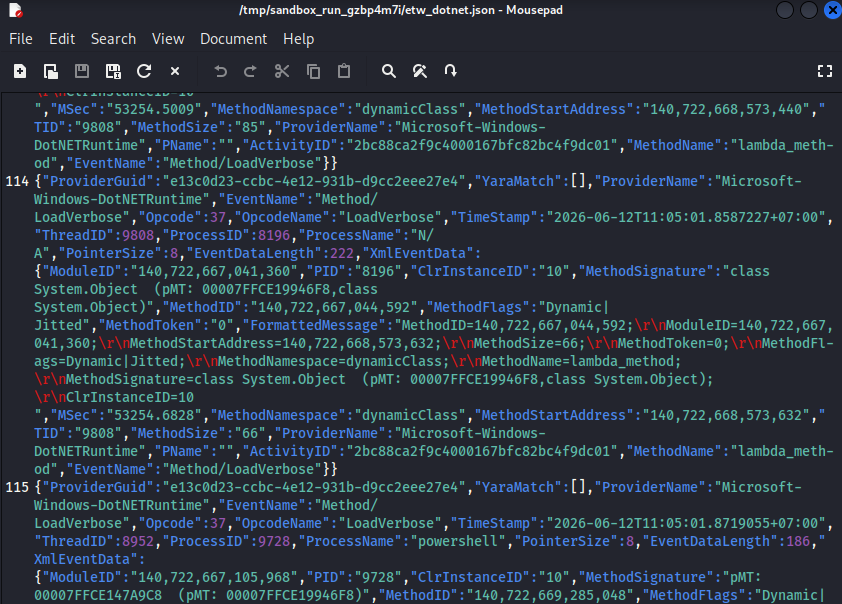
\includegraphics[width=0.8\linewidth]{Hinhve/Pic21ETWOutput.png}
\caption{Các sự kiện ETW thô về nạp assembly .NET trong tệp
  \texttt{etw\_dotnet.json} sau khi kéo từ guest về host.}
\label{fig:silketw-output}
\end{figure}
\subsection{Agent giám sát trong VM và giao tiếp với host}
\label{section:4.3.3}

Agent là ứng dụng HTTP nhẹ xây dựng trên FastAPI, lắng nghe tại
cổng~\texttt{8001}, được khởi động tự động qua Task Scheduler khi
hệ điều hành khởi động mà không yêu cầu đăng nhập. Agent đóng vai
trò lớp trung gian giữa host và các thành phần thu thập bên trong
VM, cho phép host điều khiển phiên phân tích qua API HTTP mà không
tương tác trực tiếp với giao diện Windows. HTTP REST được chọn thay
cho WinRM hay PsExec vì không yêu cầu cấu hình dịch vụ hệ thống
phức tạp và dễ mở rộng thêm endpoint.

Hình~\ref{fig:agent-swagger} cho thấy giao diện tài liệu API tự động
(Swagger UI) của Agent.
\begin{figure}[H]
\centering
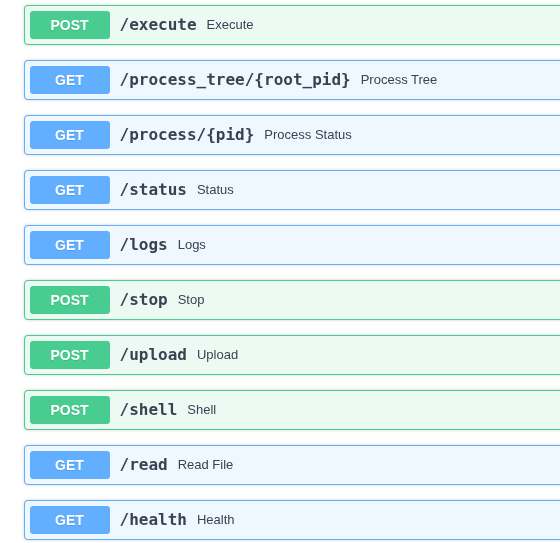
\includegraphics[width=0.5\linewidth]{Hinhve/Pic22Agent.png}
\caption{Giao diện tài liệu API tự động (Swagger UI) của Agent tại cổng~8001.}
\label{fig:agent-swagger}
\end{figure}
Toàn bộ 11~endpoint được liệt kê tại Phụ lục B.5
(Bảng~\ref{tab:agent-endpoints}). Phía host, lớp Bridge điều phối phiên:
xác nhận Agent sẵn sàng, lấy PID mẫu, tải tập lệnh thu thập lên guest
và khởi chạy; khi phiên kết thúc, các tệp nhật ký được kéo về host
phục vụ chuẩn hóa.

\subsection{Chuẩn hóa và lọc nhiễu}
\label{section:4.3.4}

Dữ liệu thô từ Sysmon và SilkETW được xử lý qua hai bộ chuẩn hóa
độc lập trước khi hợp nhất.

Bộ chuẩn hóa Sysmon ánh xạ mỗi Event ID sang tên hành vi tương ứng,
trích xuất các trường quan trọng và lọc nhiễu hạ tầng (Sysmon, Windows
Defender, VirtualBox). Việc lọc được áp dụng theo từng loại sự kiện thay
vì cắt bỏ đồng loạt, nhằm giảm nhiễu mà không làm mất hành vi thật: sự
kiện tạo tiến trình (EID~1) luôn được giữ để bảo toàn cây tiến trình; kết
nối DNS/NTP nền của \texttt{svchost.exe} (EID~3) bị loại nhưng tiến trình
này vẫn được giữ trong các trường hợp khác vì là đích tiêm mã phổ biến;
thư viện hệ thống đã ký (EID~7) bị lọc thêm vì chiếm phần lớn lượng sự
kiện nạp DLL.
Hình~\ref{fig:sysmon-normalize} minh họa kết quả chuẩn hóa một sự kiện
Sysmon EID~1 từ phiên phân tích mẫu AsyncRAT.
\begin{figure}[H]
\centering
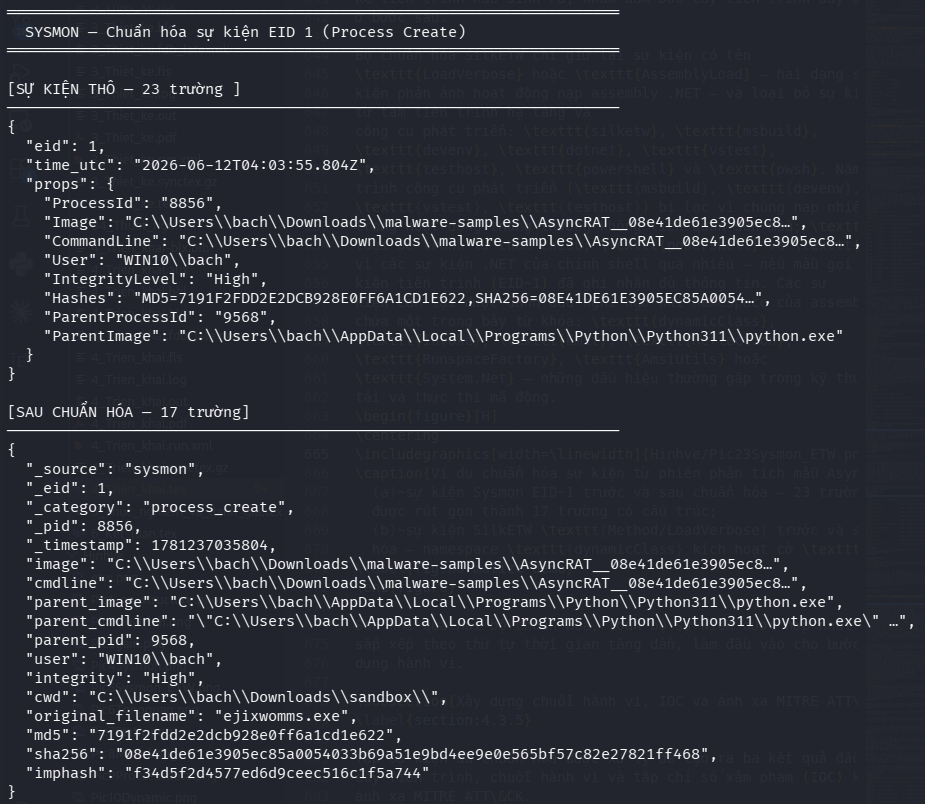
\includegraphics[width=0.95\textwidth]{Hinhve/Pic23SysmonNormalize.png}
\caption{Sự kiện Sysmon EID~1 trước và sau chuẩn hóa.}
\label{fig:sysmon-normalize}
\end{figure}
Bộ chuẩn hóa SilkETW chỉ giữ lại sự kiện \texttt{LoadVerbose} và
\texttt{AssemblyLoad} phản ánh hoạt động nạp assembly .NET, đồng thời
loại bỏ sự kiện từ tám tiến trình hạ tầng phát triển, công cụ thu thập
và trình thông dịch shell để tránh nhiễu (Phụ lục B.4,
Bảng~\ref{tab:silketw-exclude}), rồi trích xuất namespace và phương thức
được nạp. Namespace là căn cứ để bước ánh xạ MITRE
(Mục~\ref{section:4.3.5}) nhận diện kỹ thuật nạp mã phản chiếu trong bộ
nhớ (T1620) --- lớp hành vi mà Sysmon ở mức hệ điều hành không quan sát
được; bảy từ khóa namespace phản ánh nạp và thực thi mã động dùng để
khoanh vùng các sự kiện .NET đáng chú ý được liệt kê tại Phụ lục B.4
(Bảng~\ref{tab:silketw-keywords}).
Hình~\ref{fig:etw-normalize} cho thấy kết quả chuẩn hóa tương ứng cho
một sự kiện SilkETW \texttt{LoadVerbose}.
\begin{figure}[H]
\centering
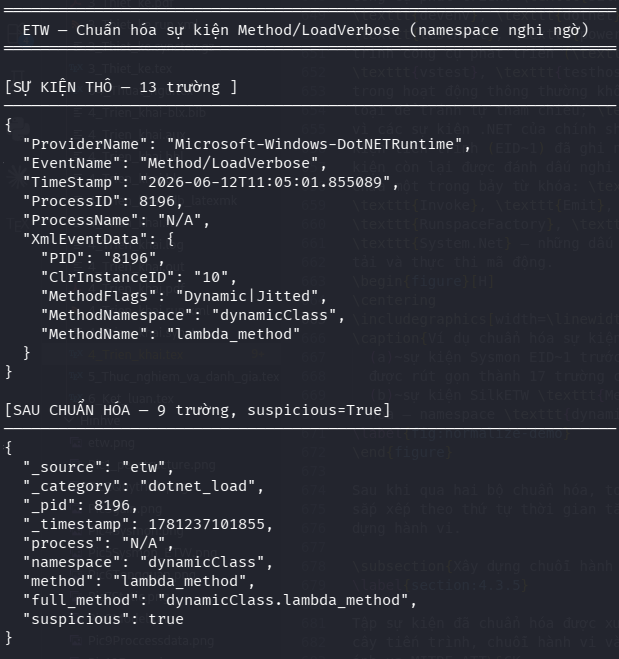
\includegraphics[width=0.65\textwidth]{Hinhve/Pic24ETWNormalize.png}
\caption{Sự kiện SilkETW \texttt{Method/LoadVerbose} trước và sau chuẩn
  hóa.}
\label{fig:etw-normalize}
\end{figure}
Sau khi qua hai bộ chuẩn hóa, sự kiện được hợp nhất và sắp xếp
theo thứ tự thời gian, làm đầu vào cho bước xây dựng hành vi.

\subsection{Xây dựng chuỗi hành vi, IOC và ánh xạ MITRE ATT\&CK}
\label{section:4.3.5}

Tập sự kiện đã chuẩn hóa được xử lý thành ba thành phần biểu diễn
hành vi --- cây tiến trình, chuỗi hành vi và tập IOC
--- rồi từ đó ánh xạ sang danh sách kỹ thuật MITRE ATT\&CK.

Cây tiến trình.
Cây được xây dựng từ sự kiện tạo tiến trình (EID~1); mỗi nút lưu
PID, tên tệp thực thi, dòng lệnh, PID cha và dấu thời gian.
27~tiến trình hệ thống thường trực được lọc theo bốn nhóm nhiễu
nền (Phụ lục B.4, Bảng~\ref{tab:tree-noise}), nhưng chỉ ẩn khỏi
cây khi toàn bộ nhánh bên dưới cũng là nhiễu — ngược lại nút cha
được giữ để bảo toàn ngữ cảnh cha–con.
Hình~\ref{fig:process-tree-example} minh họa cây tiến trình của
một mẫu phân tích sau khi lọc nhiễu.
\begin{figure}[H]
\centering
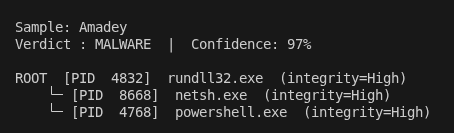
\includegraphics[width=0.95\textwidth]{Hinhve/Pic25ProcessTree.png}
\caption{Ví dụ cây tiến trình sau khi lọc nhiễu của một mẫu phân tích.}
\label{fig:process-tree-example}
\end{figure}
Chuỗi hành vi.
24~loại sự kiện chuẩn hóa được gom vào 11~nhóm hành vi theo bảng
ánh xạ cố định tại Phụ lục B.6 (Bảng~\ref{tab:event-groups}).
Mỗi nhóm ghi lại thời điểm xuất hiện đầu tiên, tổng số sự kiện, và
tối đa ba sự kiện tiêu biểu được kết xuất thành chuỗi dễ đọc (tên
tiến trình kèm dòng lệnh, địa chỉ đích, hoặc cặp nguồn–đích cho sự
kiện tiêm mã) để minh họa cụ thể mà không liệt kê toàn bộ. Toàn bộ
chuỗi được sắp xếp theo thời gian, phản ánh diễn biến hoạt động của
mẫu.
Hình~\ref{fig:behavioral-chain-example} là đầu ra chuỗi
hành vi của một mẫu cụ thể.
\begin{figure}[H]
\centering
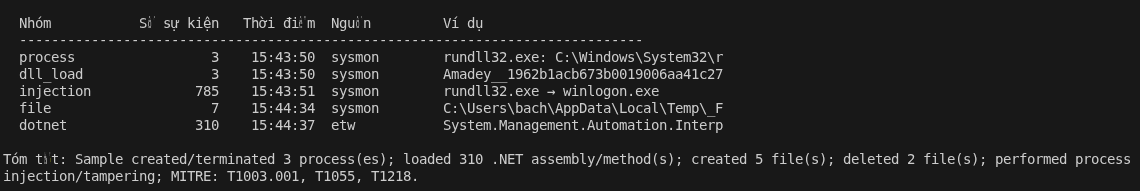
\includegraphics[width=1.0\textwidth]{Hinhve/Pic26Chain.png}
\caption{Ví dụ đầu ra chuỗi hành vi của một mẫu phân tích.}
\label{fig:behavioral-chain-example}
\end{figure}
Tập IOC.
IOC được trích xuất trong cùng vòng duyệt sự kiện, thu vào mười danh
mục: địa chỉ IP đích, tên miền, URL, tệp được tạo, tệp bị xóa, khóa
registry, câu lệnh thực thi, named pipe, PID tiến trình bị tiêm mã và
giá trị băm SHA-256. Địa chỉ IP chỉ ghi nhận khi là IP công khai; tên
miền loại trừ dịch vụ hệ thống phổ biến và được kiểm tra dấu hiệu DGA
theo entropy Shannon; URL được trích xuất bằng biểu thức chính quy từ
nội dung sự kiện. Sau khi xây dựng xong chuỗi và IOC, hệ thống tổng
hợp một đoạn tóm tắt định tính về hoạt động của mẫu trong phiên quan sát.

Ánh xạ MITRE ATT\&CK.
Hệ thống ánh xạ ATT\&CK theo 23~kỹ thuật xác định trước; khi điều kiện
thỏa mãn, kỹ thuật tương ứng được ghi nhận kèm nguồn tín hiệu
(Sysmon, SilkETW hoặc cả hai) và mức tin cậy, đưa vào báo cáo để người
phân tích cân nhắc độ tin của từng dấu hiệu. Các luật phủ ba nhóm chính: tiêm
mã và leo thang đặc quyền, cố thủ qua registry và WMI, phát hiện
kênh C2 và mạng. Bốn kỹ thuật (T1071.001, T1568.002, T1566.001 và
T1070.007) được đánh mức tin cậy trung bình do tín hiệu kích hoạt
có thể xuất hiện cả trong hoạt động hợp pháp; các kỹ thuật còn lại
được đánh mức cao. Toàn bộ 23~kỹ thuật được liệt kê tại Phụ lục B.2
(Bảng~\ref{tab:mitre-rules}).
Hình~\ref{fig:mitre-result-example} biểu diễn ví dụ kết quả ánh xạ
của một phiên phân tích thực tế.
\begin{figure}[H]
\centering
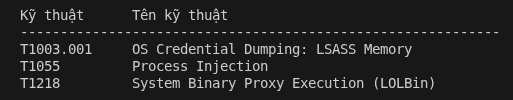
\includegraphics[width=0.95\textwidth]{Hinhve/Pic27MITRE.png}
\caption{Ví dụ kết quả ánh xạ MITRE ATT\&CK của một mẫu phân tích.}
\label{fig:mitre-result-example}
\end{figure}
\section{Triển khai pipeline tích hợp}
\label{section:4.4}

Theo thiết kế tại Mục~\ref{section:3.5}, pipeline tích hợp phối hợp
hai giai đoạn phân tích tĩnh và động để đưa ra kết luận cuối cùng và
xuất báo cáo. Triển khai tập trung vào ba khía cạnh: cơ chế thực thi
song song, quy tắc kết hợp kết quả và cấu trúc báo cáo đầu ra.

\subsection{Luồng xử lý song song}
\label{section:4.4.1}

Theo thiết kế tại Mục~\ref{section:3.5.1}, khi nhận tệp PE đầu vào,
pipeline khởi động đồng thời hai luồng qua
\texttt{ThreadPoolExecutor(max\_workers=2)}. Luồng phân tích tĩnh
(Stage~1) trích xuất vector đặc trưng từ cấu trúc PE, rút gọn xuống
384~chiều theo bộ chỉ số đã lưu và chạy mô hình LightGBM, trả về nhãn
phân loại cùng xác suất malware. Toàn bộ bước này chỉ đọc cấu trúc của
tệp trên host và không thực thi mẫu, nên hoàn tất trong vài giây và độc
lập hoàn toàn với máy ảo; nhờ đó kết quả tĩnh luôn có sẵn, kể cả với mẫu
từ chối chạy hoặc cố phát hiện sandbox để không bộc lộ hành vi.

Ngược lại, luồng phân tích động phải thực thi mẫu thật trong máy ảo
cách ly và quan sát đến hết cửa sổ thời gian định trước, nên chậm hơn
và phụ thuộc vào guest; bù lại, nó bộc lộ được các hành vi lúc chạy ---
tạo tiến trình, tiêm mã, nạp assembly .NET trong bộ nhớ --- vốn không
hiện ra khi chỉ phân tích cấu trúc tệp. Luồng này lần lượt qua ba nhóm
việc: chuẩn bị môi trường
(Stage~2–4: khôi phục snapshot, xác nhận Agent, tải mẫu), thực thi và
thu thập (Stage~5–8: ghi mốc Sysmon baseline, chạy mẫu, khởi động bộ
thu thập, chờ hết cửa sổ quan sát và kéo tệp về host), và xử lý
(Stage~9–11: chuẩn hóa sự kiện, xây dựng hành vi và IOC, đóng gói bằng
chứng). Hai luồng không phụ thuộc nhau; cả hai hoàn tất mới chuyển sang
Stage~12 tổng hợp kết quả.

Mỗi bước được bọc riêng trong khối xử lý ngoại lệ; khi lỗi xảy ra,
báo cáo vẫn được xuất với kết quả tĩnh đã có, đáp ứng yêu cầu NF4.
Hình~\ref{fig:pipeline-log} ghi lại log thực thi của pipeline trong
một phiên phân tích thực tế.
\begin{figure}[H]
\centering
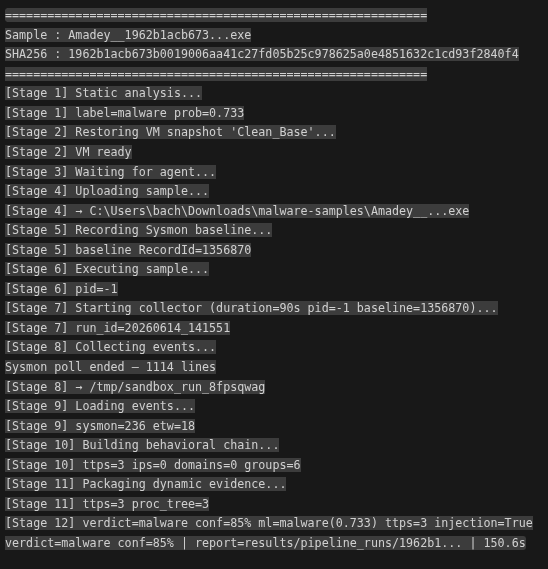
\includegraphics[width=0.95\textwidth]{Hinhve/Pic28Pipeline.png}
\caption{Log thực thi pipeline tích hợp trong một phiên phân tích.}
\label{fig:pipeline-log}
\end{figure}
\subsection{Kết hợp kết quả và xác định kết luận}
\label{section:4.4.2}

Sau khi cả hai luồng hoàn tất, hệ thống tổng hợp kết quả theo năm
quy tắc ưu tiên được liệt kê trong Bảng~\ref{tab:verdict-impl}. Tín
hiệu tiêm mã được xác định từ hai nguồn: danh sách PID tiến trình bị
tiêm trong IOC, hoặc sự xuất hiện của kỹ thuật T1055 (Process Injection)
hay T1003.001 (LSASS Memory) trong tập MITRE.

Trong toàn bộ tín hiệu thu được ở giai đoạn động, chỉ tiêm mã được dùng
làm căn cứ điều chỉnh kết luận, còn các hành vi khác (tạo tệp, ghi
registry, kết nối mạng, ánh xạ MITRE) chỉ đóng vai trò bằng chứng diễn
giải trong báo cáo. Lý do là tiêm mã có độ chính xác cao nhất: hệ thống
chỉ tính là tiêm mã khi một tiến trình mở tiến trình khác với quyền
\emph{ghi} vào bộ nhớ (kèm thao tác cấp phát vùng nhớ hoặc tạo luồng),
nên loại được các công cụ hợp pháp vốn chỉ \emph{đọc} thông tin tiến
trình; nhờ vậy tỉ lệ dương tính giả thấp (Mục~\ref{section:5.3.4}). Ngược lại,
tạo tệp, ghi khóa registry hay kết nối mạng xuất hiện phổ biến cả ở phần
mềm hợp pháp như bộ cài đặt, nên nếu dùng để đổi nhãn sẽ gây nhiều báo
động giả. Cơ chế kết hợp vì vậy bất đối xứng: tín hiệu động chỉ có thể
nâng mức nghi ngờ, không hạ một kết luận \texttt{malware} của giai đoạn
tĩnh xuống \texttt{benign}.
\begin{table}[H]
\centering
\setlength{\tabcolsep}{4pt}
\caption{Quy tắc kết hợp kết quả và tính độ tin cậy tổng hợp.}
\label{tab:verdict-impl}
\begin{tabular}{|c|p{3cm}|p{2.4cm}|l|l|}
\hline
\multicolumn{1}{|c|}{\textbf{Quy tắc}} & \multicolumn{1}{c|}{\textbf{Kết quả ML}} & \multicolumn{1}{c|}{\textbf{Tín hiệu tiêm mã}} & \multicolumn{1}{c|}{\textbf{Kết luận}} & \multicolumn{1}{c|}{\textbf{Độ tin cậy}} \\
\hline
1 & Xác suất malware $\geq 5\%$  & Có  & \texttt{malware}    & $\max(\text{ml\_prob},\, 0{,}85)$ \\
\hline
2 & Xác suất malware $< 5\%$     & Có  & \texttt{suspicious} & $0{,}65$ \\
\hline
3 & ML dự đoán malware           & Không & \texttt{malware}  & ml\_prob \\
\hline
4 & ML dự đoán benign            & Không & \texttt{benign}   & $1 - \text{ml\_prob}$ \\
\hline
5 & Không có kết quả ML          & ---   & \texttt{unknown}  & $0$ \\
\hline
\end{tabular}
\end{table}
Điều kiện ML ở hai cặp quy tắc được diễn đạt khác nhau vì chúng so với
hai ngưỡng khác nhau. Khi phát hiện tiêm mã (quy tắc~1 và~2), hệ thống
không dùng nhãn phân loại thường mà so trực tiếp xác suất malware thô với
ngưỡng hạ thấp 5\%: tín hiệu hành vi đã đủ mạnh nên chỉ cần xác suất tĩnh
vượt 5\% là kết luận \texttt{malware}. Khi không có tiêm mã (quy tắc~3
và~4), hệ thống dùng nhãn ML thường --- vốn đã được quyết định theo ngưỡng
triển khai $\tau = 0{,}33$ ngay trong bộ phân loại (Mục~\ref{section:5.2.3});
khi đó ``ML dự đoán malware'' nghĩa là xác suất vượt 0{,}33. Ngưỡng
override 5\% thấp hơn $\tau$ chính là để thu hồi những mẫu bị giai đoạn
tĩnh chấm dưới ngưỡng nhưng bộc lộ tiêm mã khi thực thi. Quy tắc~1 còn
đặt sàn độ tin cậy 85\% theo cùng lý do, ngay cả khi mô hình tĩnh cho xác
suất thấp.
Quy tắc~3 kèm thêm điều kiện: nếu phân tích động chạy thành công nhưng
không thu được tín hiệu MITRE nào và không có kết nối IP ra ngoài, hệ
thống ghi cảnh báo nghi ngờ mẫu lẩn tránh sandbox.

\subsection{Xuất báo cáo đầu ra}
\label{section:4.4.3}

Sau khi xác định kết luận, pipeline ghi kết quả ra tệp JSON trong thư
mục \texttt{results/\allowbreak pipeline\_\allowbreak runs/}. Tên tệp có dạng
\texttt{\{sha256[:12]\}\_\allowbreak\{timestamp\}\allowbreak.json} để dễ tra cứu theo mẫu
và theo thời gian. Báo cáo tổ chức theo năm nhóm trường như thiết kế
tại Mục~\ref{section:3.5.2}; tên trường thực tế của từng nhóm được
liệt kê tại Phụ lục B.7 (Bảng~\ref{tab:report-impl}).
Hình~\ref{fig:report-json} là ví dụ báo cáo JSON của một phiên
phân tích mẫu mã độc thực tế.
\begin{figure}[H]
\centering
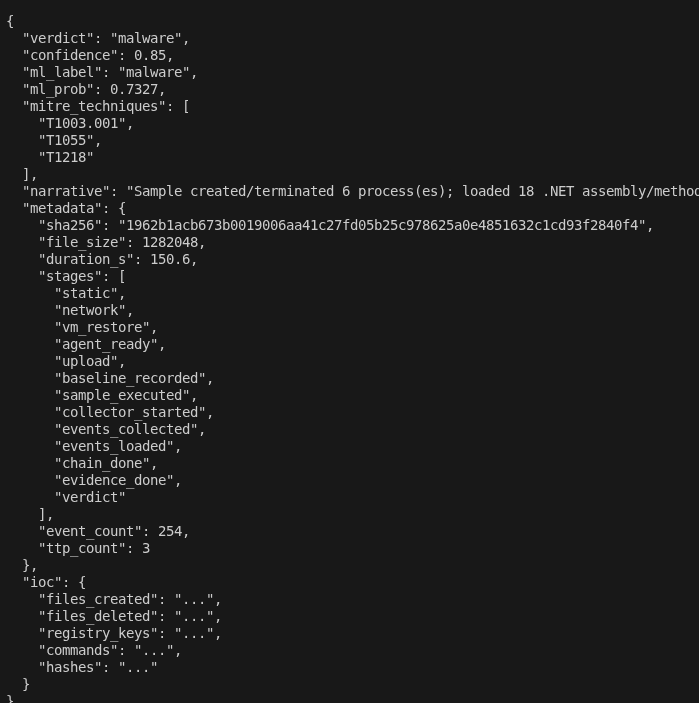
\includegraphics[width=0.95\textwidth]{Hinhve/Pic29JSON.png}
\caption{Ví dụ báo cáo JSON đầu ra của một phiên phân tích mẫu mã độc.}
\label{fig:report-json}
\end{figure}
\section{Giao diện web demo}
\label{section:4.5}

Server Flask lắng nghe tại cổng~\texttt{5001}, cung cấp tám endpoint REST
và phát sự kiện tiến trình phân tích qua SSE; mỗi yêu cầu phân tích được
xử lý bởi một luồng nền độc lập kèm hàng đợi sự kiện riêng. Danh sách
endpoint và loại sự kiện SSE được trình bày tại Phụ lục B.3
(Bảng~\ref{tab:demo-endpoints}, Bảng~\ref{tab:sse-events}). Giao diện phía
client được tổ chức thành một tệp CSS và bốn tệp JavaScript, phân theo
chức năng: điều hướng, xử lý SSE, danh sách báo cáo và kết xuất chi tiết.
Giao diện được tổ chức thành bốn trang chính, lần lượt trình bày dưới đây.

Trang Analyze (Hình~\ref{fig:demo-analyze}).
Người dùng tải mẫu \texttt{.exe}/\texttt{.dll} qua vùng kéo-thả rồi
tinh chỉnh các thông số môi trường: máy ảo và snapshot, địa chỉ Agent,
thời lượng quan sát (mặc định 120~giây) và thông tin đăng nhập guest. Ba
tùy chọn bật/tắt cho phép bỏ qua phân tích tĩnh, động hoặc tầng mạng để
chạy riêng từng phần. Nhấn ``Run Analysis'' để khởi chạy.
\begin{figure}[H]
\centering
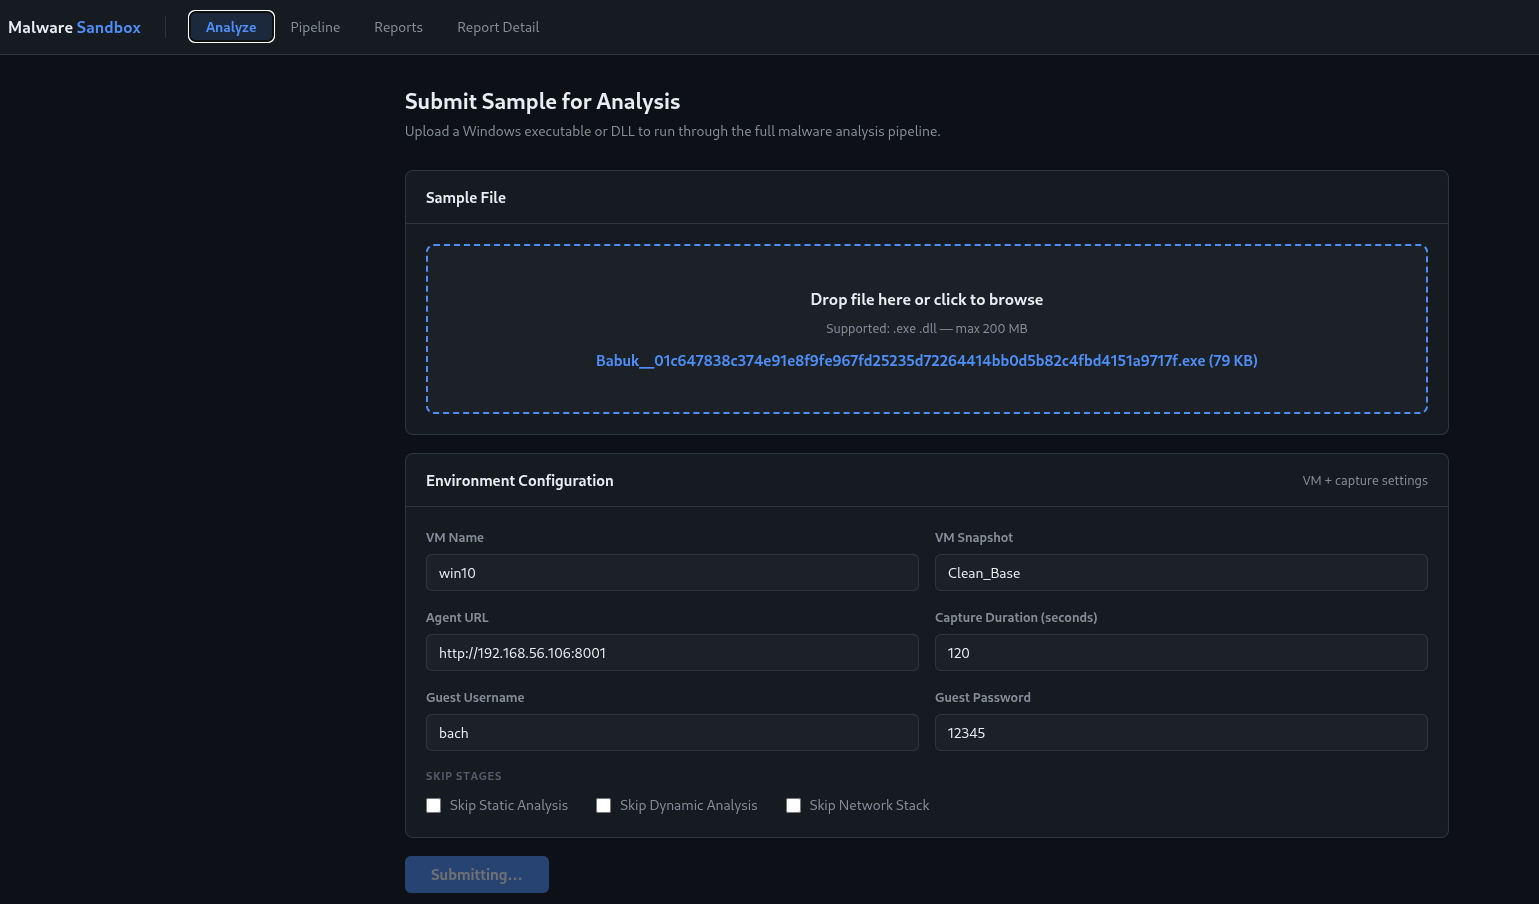
\includegraphics[width=0.9\textwidth]{Hinhve/Pic30MainUI.png}
\caption{Trang Analyze: vùng kéo-thả và biểu mẫu cấu hình môi trường phân tích.}
\label{fig:demo-analyze}
\end{figure}
Trang Pipeline (Hình~\ref{fig:demo-pipeline}).
Giao diện cập nhật 12 giai đoạn qua luồng SSE và xuất báo cáo tự động
khi phân tích hoàn tất; nút ``Stop Pipeline'' cho phép dừng phiên
giữa chừng.
\begin{figure}[H]
\centering
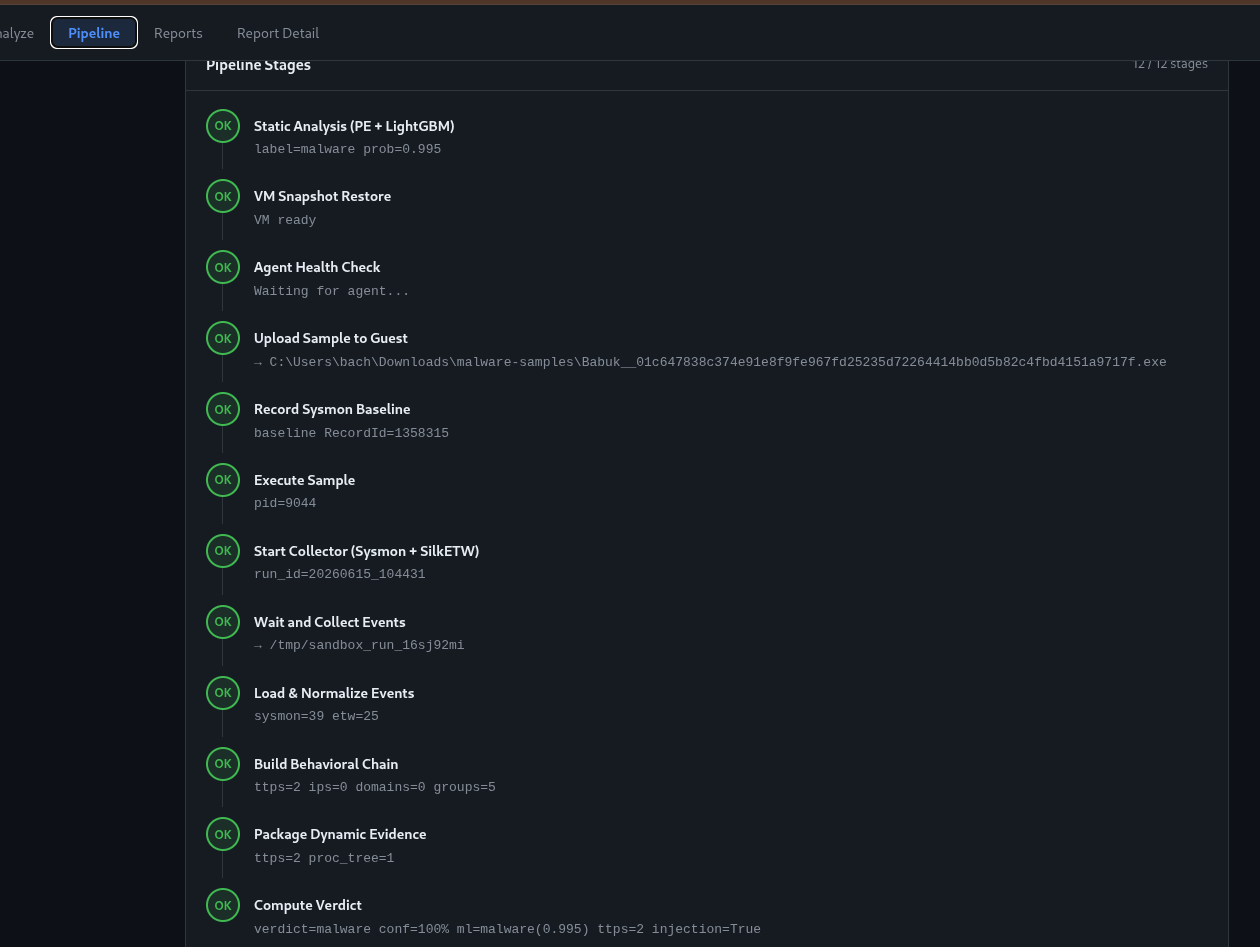
\includegraphics[width=0.9\textwidth]{Hinhve/Pic31Pipeline.png}
\caption{Trang Pipeline: 12~giai đoạn phân tích.}
\label{fig:demo-pipeline}
\end{figure}
Trang Reports (Hình~\ref{fig:demo-reports}).
Bảng liệt kê các phiên phân tích đã lưu, sắp xếp theo thời gian giảm dần;
mỗi hàng hiển thị verdict, tên mẫu, tiền tố SHA-256, số cảnh báo/lỗi,
số kỹ thuật MITRE, số sự kiện, thời lượng và thời điểm phân tích.
Nhấn vào một hàng để chuyển sang trang báo cáo chi tiết.
\begin{figure}[H]
\centering
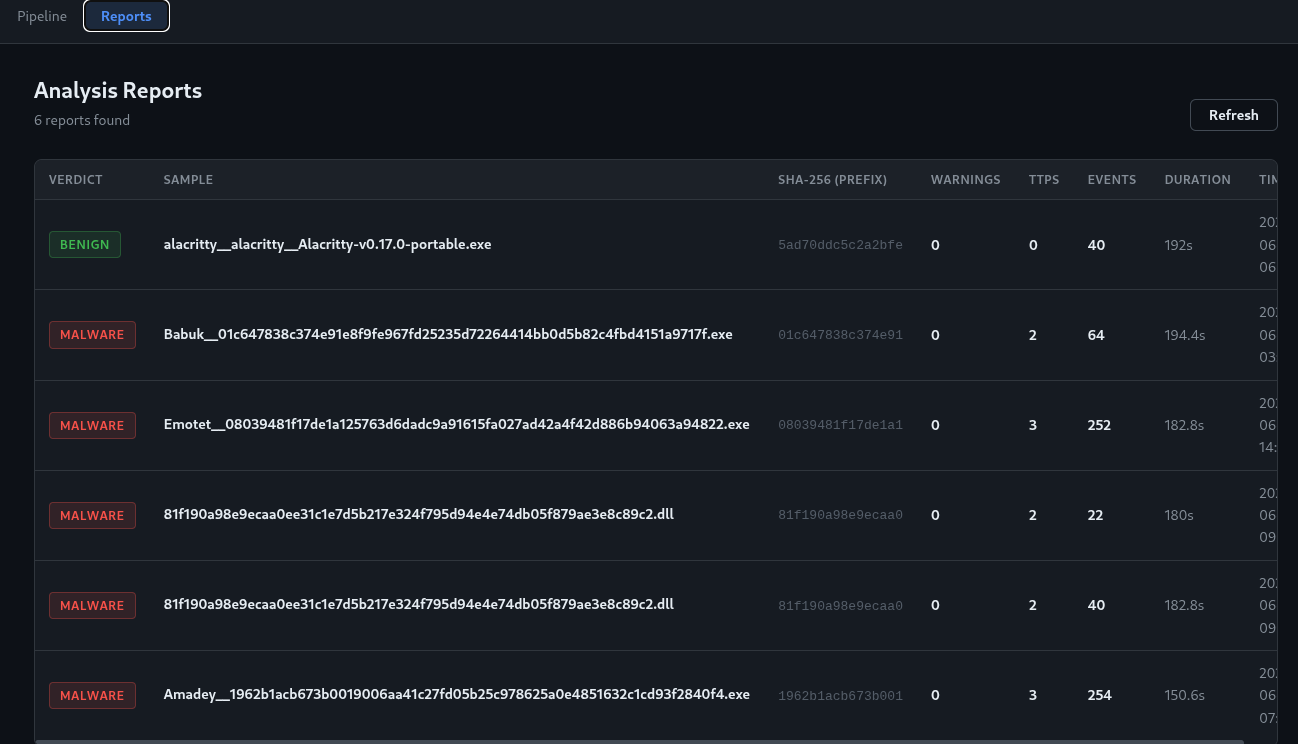
\includegraphics[width=0.9\textwidth]{Hinhve/Pic32Report.png}
\caption{Trang Reports: bảng tổng hợp kết quả các phiên phân tích đã lưu.}
\label{fig:demo-reports}
\end{figure}
Trang Report Detail (Hình~\ref{fig:demo-report-detail}).
Trang trình bày kết quả phân tích chi tiết của một phiên, gồm phần
kết luận (verdict, nhãn ML, độ tin cậy) và các tab dữ liệu: Warnings,
MITRE ATT\&CK, Indicators of Compromise, Behavioral Chain và Metadata;
tab Process Tree chỉ xuất hiện khi phiên thu được dữ liệu cây tiến trình.
\begin{figure}[H]
\centering
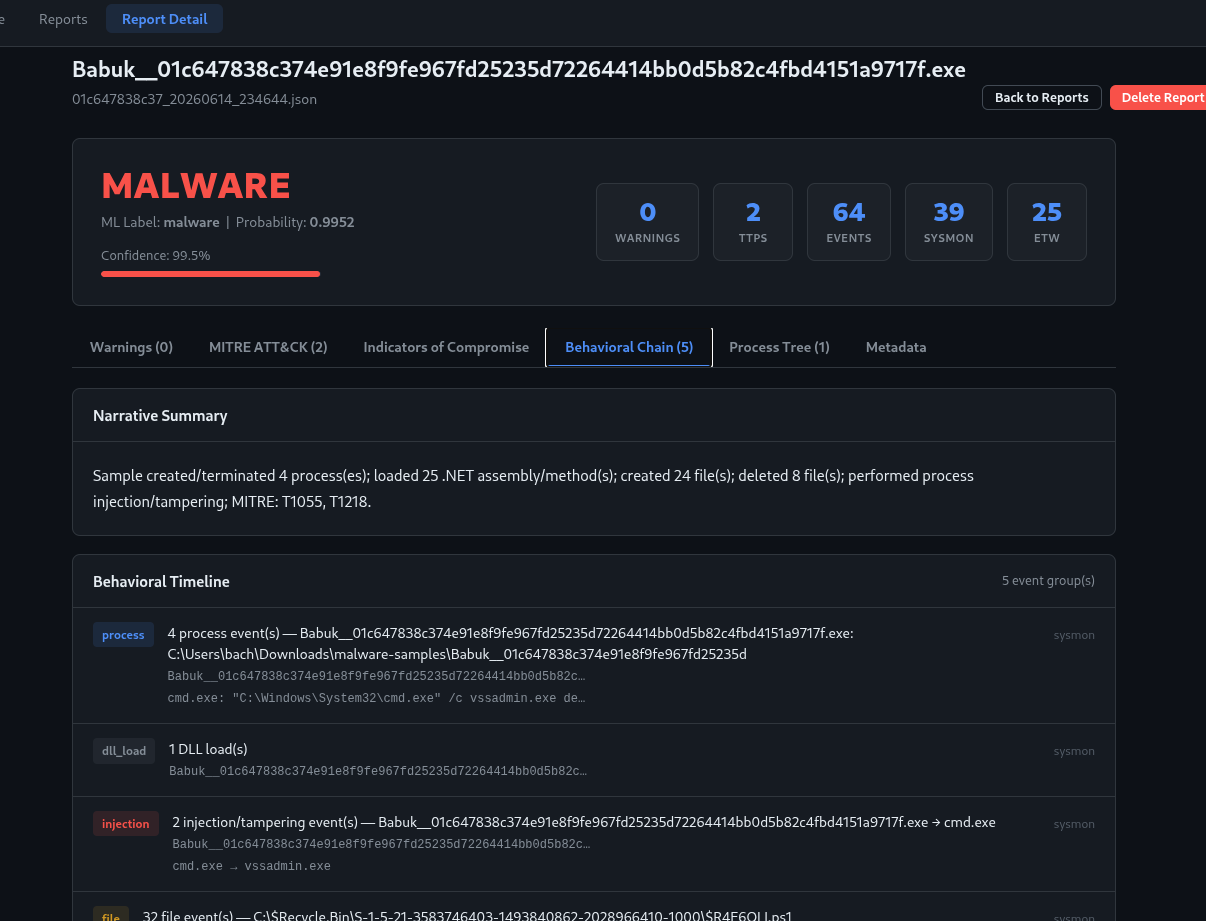
\includegraphics[width=0.9\textwidth]{Hinhve/Pic33ReportDetail.png}
\caption{Trang Report Detail: báo cáo chi tiết 1 mẫu phân tích.}
\label{fig:demo-report-detail}
\end{figure}

Kết quả triển khai là một pipeline vận hành tự động hoàn toàn từ khâu
nhận tệp PE đến khâu xuất báo cáo JSON: giai đoạn tĩnh chạy trên host
song song với giai đoạn động trong máy ảo, hai luồng sự kiện Sysmon và
ETW được chuẩn hóa rồi hợp nhất, và kết quả được hiển thị qua giao diện
web. Hiệu năng và độ chính xác của hệ thống được đánh giá ở
Chương~\ref{chapter:Experiment}.

\end{document}
